% !TEX root = ../main.tex
%% Section 5: Evaluation

\section{Evaluation}\label{sec:evaluation}

\subsection{Experimental Setup}\label{sec:setup}

We conducted a campaign of 3 attacker variants $\times$ 3 operating points $\times$ 5 random seeds = 45 planned experiments, each running for 300 seconds (5 minutes) of simulation time with fresh federation restart between experiments to avoid HELICS time-synchronization deadlocks.
Of the 45 planned experiments, 37 completed successfully (82\%); 8 failed due to HELICS timeout errors, with seed~2 systematically failing across multiple variants (a reproducible interaction between specific random number sequences and HELICS federation timing), yielding final sample sizes of $N = 5$ for AI-V1 at all operating points, $N = 3$--$4$ for Random, and $N = 3$--$4$ for AI-V2.
Three Docker containers ran in parallel (one per operating point), each hosting the full HELICS federation with GridPACK, two GridLAB-D instances, the v2 controller, and the MCP attacker server; attacker scripts ran on the host machine communicating with the MCP server via HTTP on port~5100.
The primary metric is Threshold Violation Duration (TVD); secondary metrics include cycle position (average position in the controller's 10-second observation cycle where 0.0 is optimal) and unique EVs targeted (measuring diversification). See Table~\ref{tab:raw-data} in Appendix~B for per-experiment data.
All experiments use a single grid topology (IEEE 123-node), a single LLM (Qwen 3.5-122B), and a single defense mechanism; results may vary under different configurations.

\subsection{Main Results}\label{sec:results}

Table~\ref{tab:main_results} presents the complete results across all nine experimental cells.
At Hour~4 (low load, ${\sim}$720~kW headroom), AI-V2 achieves TVD = $135 \pm 30$~s compared to Random's $60 \pm 49$~s, while AI-V1 achieves only $48 \pm 27$~s (lower than random) due to its timing gate consuming attack opportunities while its single-target fixation (mean 1.6 unique EVs vs.\ V2's 3.8) limits cumulative load impact.
At Hour~7 (medium load, ${\sim}$497~kW headroom), the differentiation is sharpest: AI-V2 achieves TVD = $180 \pm 0$~s with perfect consistency across all seeds, AI-V1 achieves $120 \pm 0$~s with consistent but lower performance (targeting only 1.0 unique EVs), and Random achieves $75 \pm 30$~s.
At Hour~14 (high load, base load exceeding threshold by 1290~kW), all three variants achieve identical TVD = $295 \pm 0$~s (the full experiment duration minus startup transients) because the controller cannot reduce feeder power below the threshold even with all EVs shed, rendering attacker strategy irrelevant.

\begin{table*}[t]
  \caption{Main results and evaluation validity gap across operating points (mean $\pm$ std). TVD: threshold violation duration (seconds $\geq$ 4200~kW). Unique EVs: distinct EV stations targeted. Cycle pos.: mean position in controller's 10-second cycle (0.0 = optimal). EVG: ratio of variant TVD to Random TVD.}\label{tab:main_results}
  \centering
  \small
  \begin{tabular}{@{}llccccccc@{}}
    \toprule
    \textbf{OP} & \textbf{Variant} & \textbf{N} & \textbf{TVD (s)} & \textbf{Unique EVs} & \textbf{Cycle pos.} & \textbf{EVG} & \textbf{$p$} & \textbf{$d$} \\
    \midrule
    \multirow{3}{*}{Hr\,4}
      & Random & 4 & $60 \pm 49$  & 2.0 & 0.08 & ---          & ---     & --- \\
      & AI-V1  & 5 & $48 \pm 27$  & 1.6 & 0.00 & 0.80$\times$ & 0.710   & 0.28 \\
      & \textbf{AI-V2}  & \textbf{4} & $\mathbf{135 \pm 30}$  & \textbf{3.8} & \textbf{0.00} & \textbf{2.25$\times$} & \textbf{0.020*}  & \textbf{1.85} \\
    \midrule
    \multirow{3}{*}{Hr\,7}
      & Random & 4 & $75 \pm 30$  & 2.0 & 0.08 & ---          & ---     & --- \\
      & AI-V1  & 5 & $120 \pm 0$  & 1.0 & 0.00 & 1.60$\times$ & 0.038*  & 1.80 \\
      & \textbf{AI-V2}  & \textbf{4} & $\mathbf{180 \pm 0}$   & \textbf{4.0} & \textbf{0.00} & \textbf{2.40$\times$} & $\mathbf{<}$\textbf{0.001**} & \textbf{4.95} \\
    \midrule
    \multirow{3}{*}{Hr\,14}
      & Random & 3 & $295 \pm 0$  & 2.0 & 0.11 & ---          & ---     & --- \\
      & AI-V1  & 5 & $295 \pm 0$  & 1.0 & 0.00 & 1.00$\times$ & ---     & 0.00 \\
      & AI-V2  & 3 & $295 \pm 0$  & 4.0 & 0.00 & 1.00$\times$ & ---     & 0.00 \\
    \bottomrule
    \multicolumn{9}{@{}l}{\footnotesize * $p < 0.05$; ** $p < 0.001$. One-sided Welch's $t$-test.}
  \end{tabular}
\end{table*}

\subsection{Analysis}\label{sec:analysis}

\paragraph{Finding 1: The EVG is real, significant, and condition-dependent.}
At both operating points where the controller has capacity to respond (Hours~4 and~7), AI-V2 achieves 2.25--2.40$\times$ the violation duration of the Random baseline, with large effect sizes (Cohen's $d = 1.85$--$4.95$) that indicate practically meaningful differences.
In concrete terms, a security evaluation using only the non-adaptive baseline used in this study at Hour~7 would report the progressive-shedding controller as limiting violations to 75~seconds, while the same controller permits 180~seconds of violation against a strategy-aware adaptive attacker under identical resource constraints, an overestimation of defense effectiveness by a factor of~2.4.
The EVG varies systematically with grid headroom, following an inverted-U pattern: it is highest at Hour~7 (2.40$\times$) where moderate headroom provides enough space for adaptive strategy to differentiate but enough stress for violations to occur, somewhat lower at Hour~4 (2.25$\times$) where large headroom limits even V2's ability to trigger violations, and collapses to 1.0$\times$ at Hour~14 where no headroom remains.
Hour~14 serves as a ceiling case: because base load alone exceeds the threshold, attacker actions do not change TVD, and $\text{EVG} = 1.0$ by construction. This is consistent with the expectation that the gap reflects attacker capability rather than simulation artifacts.
This condition-dependence mirrors Nasr et al.'s~\cite{nasr2025attacker} finding in LLM security that the gap between static and adaptive evaluation varies with defense difficulty, a pattern that appears to generalize across security domains.

\paragraph{Finding 2: The AI-V2 prompt package outperforms AI-V1; timing alone is insufficient.}
Both AI variants achieve identical, perfect micro-timing at all operating points: cycle position 0.00 and micro-timing score 100, meaning every LLM-issued attack arrives immediately after the controller acts, exploiting the full 10-second observation window; in this setup, timing exploitation is straightforward for both variants given access to the controller's observation schedule.
The observed V2-vs-V1 gap manifests primarily as improved target diversification: V2 consistently targets 3.8--4.0 unique EVs across all operating points while V1 targets 1.0--1.6, with very large separation on the unique-EVs metric (e.g., $d = 4.07$ at Hour~4; zero-variance separation at Hours~7 and~14, $p < 0.001$). However, the current design does not isolate which prompt components cause that behavior.
Because AI-V2 adds domain knowledge, diversification guidance, dynamic attack-history context, and fixed max-power behavior simultaneously (Table~\ref{tab:variants}), the current study demonstrates but does not isolate which of these factors drives the improvement; ablation of individual prompt components is left to future work.
This dominance arises from the interaction between the additive power accumulation model and the progressive-shedding controller: the controller must shed each attacked EV in a separate 10-second cycle, so $N$ diversified attacks create a violation that requires $N$ controller cycles ($10N$ seconds) to resolve, whereas $N$ attacks on the same EV create a violation resolvable in a single cycle.
The sharpest result is V1's underperformance at Hour~4 (EVG = 0.80$\times$, below the random baseline), where V1's timing gate causes it to wait for high micro-timing scores rather than attacking immediately, consuming scarce time within the 300-second window; combined with its persistent single-target fixation (attacking EV1 exclusively in most seeds), V1 executes fewer effective attacks than the random baseline, which at least achieves accidental diversification (mean 2.0 unique EVs).
We note that AI-V1 also experienced approximately 30\% safety refusal rate from the LLM's guardrails, reducing its effective attack rate; V1's lower TVD is therefore partly attributable to missed attack opportunities, though its single-target fixation is visible even in successful attacks (mean 1.0--1.6 unique EVs vs.\ V2's 3.8--4.0).
V1 achieved locally optimal timing on every attack, yet its cumulative impact was lower than random. The gap is attributable to single-target fixation rather than timing quality, indicating that CPS red-teaming prompts must encode system dynamics (power accumulation, controller response) rather than protocol-level timing alone.
For defenders, this implies that attacks requiring multi-step physical reasoning (accumulating load across diverse targets) are qualitatively different from timing exploits and may require different detection strategies.

\paragraph{Finding 3: Strategic prompting produces deterministic, reproducible behavior.}
AI-V2 exhibits zero TVD variance ($\sigma = 0$) at Hour~7 and low variance ($\sigma = 30$~s) at Hour~4 across all seeds, following a near-identical attack sequence everywhere: EV1 $\rightarrow$ EV2 $\rightarrow$ EV3 $\rightarrow$ EV4, each at 1500~kW, each at cycle position 0.00. The strategic prompt produces highly consistent behavior in this setup (Fig.~\ref{fig:timelines}).
In contrast, AI-V1 shows moderate variance at Hour~4 ($\sigma = 27$~s) and zero variance at Hour~7 ($120 \pm 0$~s across all seeds), but this consistency reflects persistent single-target fixation rather than strategic reliability, since V1 consistently targets only 1.0 unique EVs at Hour~7.
The mechanism is the dynamic strategic context in V2's prompt---the shrinking unattacked-EV list and explicit diversification instruction anchor the LLM's target selection, overriding the model's tendency toward default or habitual choices (EV1 fixation) that dominate V1's behavior.

\begin{figure}[t]
  \centering
  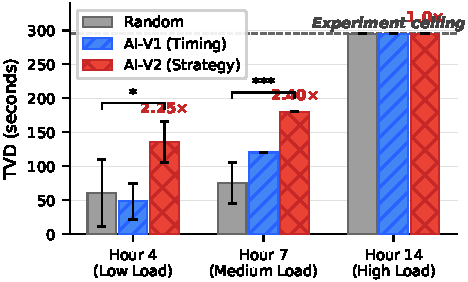
\includegraphics[width=\columnwidth]{figures/fig2_evg_barchart.pdf}
  \caption{Evaluation validity gap across operating points. AI-V2 achieves EVG = 2.25--2.40$\times$ where the controller can respond (Hours~4 and~7) and EVG = 1.0$\times$ at the ceiling operating point (Hour~14).}
  \label{fig:evg_bars}
\end{figure}

\begin{figure}[t]
  \centering
  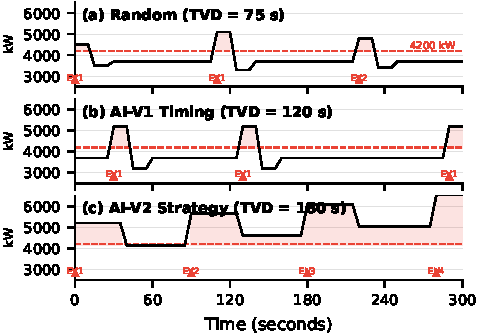
\includegraphics[width=\columnwidth]{figures/fig3_timelines.pdf}
  \caption{Attack timelines at Hour~7. AI-V2 systematically sweeps EV1--EV4 at 1500~kW; AI-V1 fixates on EV1; Random scatters attacks across targets at varying power levels.}
  \label{fig:timelines}
\end{figure}

\subsection{Limitations}\label{sec:limitations}

Several factors scope the conclusions of this study. Sample sizes are small and unbalanced across cells ($N = 3$--$5$) because 8 of 45 planned runs failed due to HELICS timeouts, which limits precision even though the observed effect sizes are large. The experiments use a single grid topology (IEEE 123-node), a single LLM (Qwen~3.5-122B), and estimate EVG using a Random baseline as the static comparator; a stronger hand-crafted static attack could narrow the measured gap. Because AI-V2 modifies multiple prompt components simultaneously (domain knowledge, diversification guidance, attack history, and fixed max-power), the current design demonstrates but does not isolate the contribution of each factor. AI-V1 experienced approximately 30\% safety refusal rate from the LLM's guardrails, which partly confounds its lower TVD with missed attack opportunities, though its single-target fixation is visible even in successful attacks.
